\chapter{Physique} \label{physique}
\section{Capteurs}\label{physiqueCapteurs}
Un transducteur est un dispositif convertissant une grandeur physique
en une autre ; par exemple une onde lumineuse en signal nerveux
(vision animale) ou signal électrique (photorécepteur).\\
Plus spécifiquement, un capteur est un dispositif qui transforme une
grandeur physique d'entrée, appelée mesurande \(\left[m\right]\), en un signal
exploitable de nature électrique (en général) appelée réponse \(\left[s\right]\).

\begin{minipage}{0.49\textwidth}
    \begin{figure}[H]
        \centering
        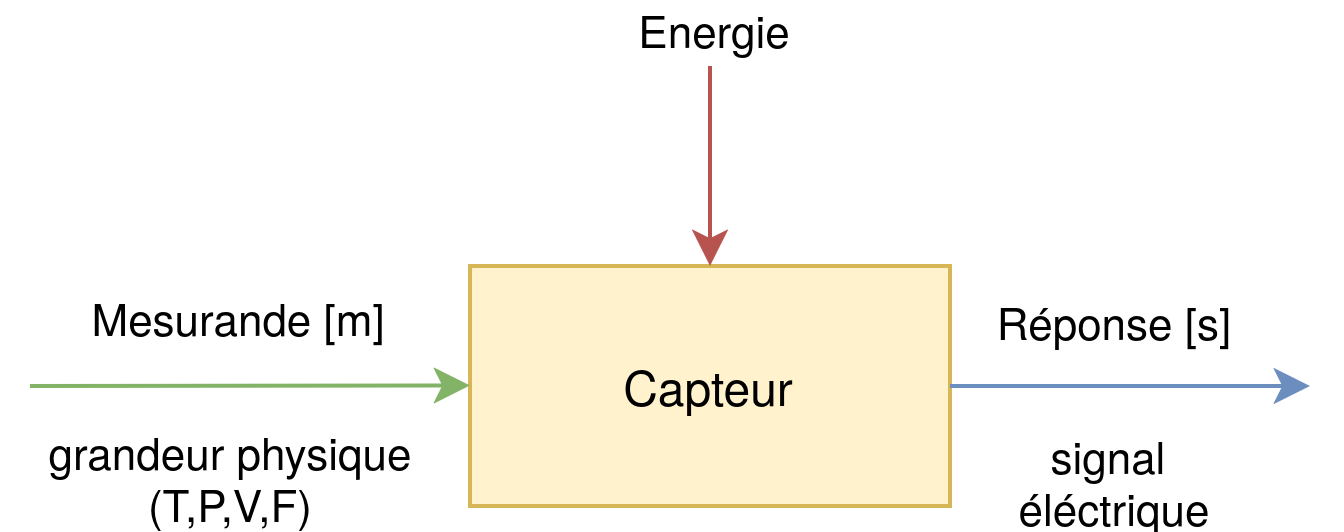
\includegraphics[width=0.9\textwidth]{capteur}
        \caption{Diagramme d'un capteur}
        \label{figCapteur}
    \end{figure}
\end{minipage}
\begin{minipage}{0.5\textwidth}
    \resizebox{\linewidth}{!}{%
    \begin{tikzpicture}
        \begin{axis}[
            axis x line=bottom,axis y line = left,
            ticks=none,
            xmax = 12,
            ymax = 10, 
            ylabel = Signal de sortie,
            xlabel = Mesurande,
        ]
            
            \addplot+[smooth, mark=none,] coordinates
              {(1,0) (2,2) (4,3) (8,8) (12,9)};
            \addplot[dashed, samples=50, smooth,domain=0:6,gray] coordinates {(2,0)(2,9)}node[above,pos=1] {seuil};
            \addplot[dashed, samples=50, smooth,domain=0:6,gray] coordinates {(6,0)(6,5.55)}node[right,pos=0.5] {m};
            \addplot[dashed, samples=50, smooth,domain=0:6,gray] coordinates {(0,5.5)(5.8,5.5)}node[above,pos=0.5] {s};
            \addplot[dashed, samples=50, smooth,domain=0:6,gray] coordinates {(8,0)(8,9)};
            \draw[<->, gray] (axis cs:2,8) -- (axis cs:8,8) node[above, pos=0.5] {\parbox{\widthof{another}}{\small\centering plage de \\ mesure }};
            \addplot[dashed, samples=50, smooth,domain=0:6,gray] coordinates {(10,0)(10,8.8)}node[above,pos=1.01] {saturation};
          \end{axis}
    \end{tikzpicture}%
    }
    \captionof{figure}{Caractéristique d'un capteur}
    \label{figCaracteristique}
\end{minipage}

Le \textbf{mesurande} \( m \) représente la grandeur physique à mesurer, comme la
température, la pression, la vitesse ou la force. La \textbf{réponse} \( s \) 
du capteur correspond à une grandeur électrique en sortie. La \textbf{caractéristique de transfert} 
\( s = f(m) \) établit la relation entre le mesurande et la réponse du capteur.
Elle est propre au capteur et à son environnement de mesure.\par
Parmi toutes les grandeurs physiques, la température est l'une des plus couramment
mesurées, car elle influence directement les propriétés de la matière.

Un capteur de température se caractérise par plusieurs paramètres. 
L'\textbf{étendue de mesure} (E.M) correspond à l'intervalle entre les valeurs 
extrêmes pouvant être mesurées (\( E.M = m_{\max} - m_{\min} \)). La 
\textbf{résolution} est la plus petite variation détectable. Enfin, la 
\textbf{sensibilité} représente la variation du signal de sortie en réponse à 
une variation du mesurande, correspondant à la pente de la courbe caractéristique 
du capteur.

\begin{minipage}{0.3\textwidth}
    \[
        S(m) = \left(\frac{\Delta s}{\Delta m}\right)_{m_0}
    \]
\end{minipage}
\begin{minipage}{0.69\textwidth}
    \resizebox{\linewidth}{!}{%
    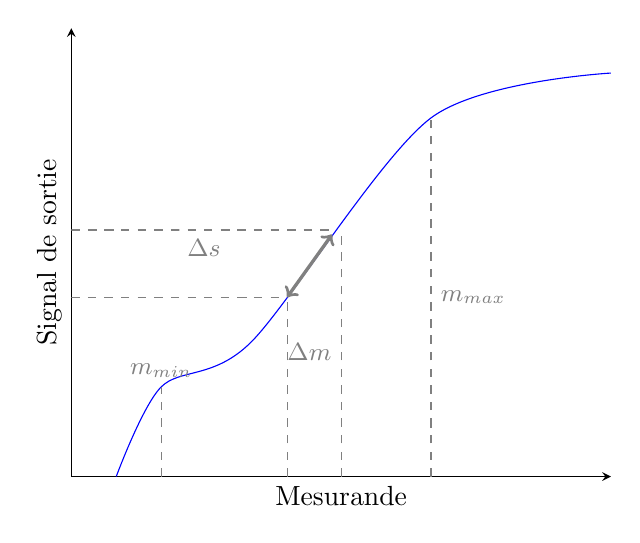
\begin{tikzpicture}
        \begin{axis}[
            axis x line=bottom,axis y line = left,
            ticks=none,
            xmax = 12,
            ymax = 10, 
            ylabel = Signal de sortie,
            xlabel = Mesurande,
        ]
            
            \addplot+[smooth, mark=none,] coordinates
              {(1,0) (2,2) (4,3) (8,8) (12,9)};
            \addplot[dashed, samples=50, smooth,domain=0:6,gray] coordinates {(2,0)(2,2)}node[above,pos=1] {\small\(m_{min}\)};
            \addplot[dashed, samples=50, smooth,domain=0:6,gray] coordinates {(4.8,0)(4.8,4)};
            \addplot[dashed, samples=50, smooth,domain=0:6,gray] coordinates {(6,0)(6,5.55)}node[left,pos=0.5] {\small\(\Delta m\)};
            \addplot[dashed, samples=50, smooth,domain=0:6,gray] coordinates {(0,4)(4.8,4)};
            \addplot[dashed, samples=50, smooth,domain=0:6,gray] coordinates {(0,5.5)(5.9,5.5)}node[below,pos=0.5] {\small\(\Delta s\)};
            \addplot[dashed, samples=50, smooth,domain=0:6,gray] coordinates {(8,0)(8,8)}node[right,pos=0.5] {\small\(m_{max}\)};
            \draw[<->, very thick, gray] (axis cs:4.8,4) -- (axis cs:5.8,5.4);
        \end{axis}
    \end{tikzpicture}%
    }
    \captionof{figure}{Sensibilité d'un capteur}
    \label{fig:sensibilite}
\end{minipage}

La \textbf{linéarité} d'un capteur définit la plage dans laquelle la 
\textbf{sensibilité} (variation du signal de sortie par rapport à la variation 
du mesurande) reste constante. Autrement dit, dans cette zone, la relation entre 
l'entrée (\( m \), la grandeur physique mesurée) et la sortie (\( s \), la
réponse du capteur) peut être approximée par une fonction affine.\par

\begin{figure}[!ht]
    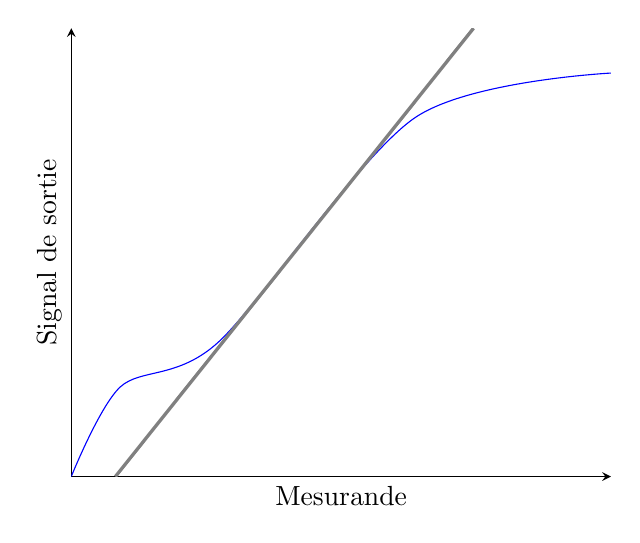
\begin{tikzpicture}
        \begin{axis}[
            axis x line=bottom,axis y line = left,
            ticks=none,
            xmax = 12,
            ymax = 10, 
            ylabel = Signal de sortie,
            xlabel = Mesurande,
        ]
            
            \addplot+[smooth, mark=none,] coordinates
              {(1,0) (2,2) (4,3) (8,8) (12,9)};
            \draw[very thick, gray] (axis cs:1.9,0) -- (axis cs:9.2,10);
        \end{axis}
    \end{tikzpicture}
    \caption{Linéarité d'un capteur}
    \label{figLineaire}
\end{figure}

Bien que la linéarité facilite l'interprétation des mesures et simplifie les 
traitements électroniques et numériques, elle limite la plage de mesure utilisable. 
En dehors de cette zone linéaire, le capteur peut présenter une 
\textbf{sensibilité variable}, c'est-à-dire que la relation entre \( s \) et
\( m \) devient non linéaire, rendant les mesures plus complexes à interpréter 
et nécessitant des corrections. Il est alors nécessaire
d'étalonner le capteur ou d'appliquer des algorithmes de compensation pour 
corriger les erreurs de linéarité lorsqu'on travaille en dehors de cette zone 
idéale.

La \textbf{précision} d'un capteur est définie par deux critères essentiels : 
la \textbf{fidélité} et la \textbf{justesse}.  

Lorsque l'on effectue \( n \) mesures d'un même mesurande dans des conditions 
identiques, la \textbf{valeur vraie} du mesurande est notée \( X_v \), tandis 
que les valeurs mesurées sont notées \( X_i \). La \textbf{valeur moyenne} des 
mesures est définie par :  

\[
X_m = \frac{\sum_{i} X_i}{n}
\]

La \textbf{fidélité} d'un capteur correspond à sa capacité à donner des 
résultats cohérents lors de mesures répétées. Elle est évaluée par 
l'\textbf{écart-type} \( \sigma \), qui traduit la dispersion des valeurs 
mesurées autour de la moyenne \( X_m \) :  

\[
\sigma = \sqrt{\frac{\sum_{i} (X_i - X_m)^2}{n-1}}
\]

Un capteur est considéré comme \textbf{fidèle} si son écart-type est faible, 
garantissant ainsi une bonne répétabilité des mesures. Toutefois, cela ne 
signifie pas nécessairement que les mesures sont proches de la valeur vraie.  

La \textbf{justesse} reflète quant à elle l'écart entre la valeur moyenne 
\( X_m \) et la valeur vraie \( X_v \). Un capteur est dit \textbf{juste} si 
\( X_m \) est proche de \( X_v \), même si ses mesures individuelles présentent 
une certaine dispersion.  

Enfin, un capteur est qualifié de \textbf{précis} lorsqu'il est à la fois 
\textbf{fidèle} et \textbf{juste}. Autrement dit, un capteur précis fournit 
des mesures répétables (fidélité) dont la moyenne est proche de la valeur vraie 
(justesse).

Les \textbf{grandeurs d'influence} sont des paramètres physiques, autres que la 
mesurande, dont la variation peut affecter la réponse d'un capteur. Parmi elles, 
la \textbf{température} peut modifier les caractéristiques électriques, 
mécaniques ou dimensionnelles du capteur, tandis que la \textbf{pression} et les
\textbf{vibrations} peuvent induire des déformations et des contraintes altérant 
ses performances. L'\textbf{humidité}, quant à elle, influence les propriétés 
électriques, telles que la constante diélectrique ou la résistivité, et peut 
dégrader l'isolation électrique. Enfin, un \textbf{champ magnétique} variable 
peut générer une force électromotrice d'induction, tandis qu'un champ statique 
peut modifier la résistivité des matériaux.  

Une autre grandeur d'influence est la \textbf{tension d'alimentation}, qui peut 
impacter directement la grandeur de sortie du capteur en modifiant son amplitude
ou sa fréquence. L'effet des grandeurs d'influence se manifeste généralement par 
un \textbf{décalage du zéro} (offset) ou une \textbf{dérive de la sensibilité}. 
Pour minimiser ces perturbations, plusieurs solutions existent : 
\textbf{réduire} les grandeurs d'influence par des dispositifs spécifiques 
(table anti-vibration, blindages magnétiques, etc.), \textbf{stabiliser} ces 
grandeurs à des valeurs connues et maîtrisées, ou encore \textbf{compenser} leur 
effet en utilisant des montages adaptés, comme le \textbf{pont de Wheatstone} ou 
un \textbf{montage différentiel}.

\section{Classification des capteurs}\label{physique:capteurs:classification}

Les capteurs peuvent être classés en fonction de la nature de leur grandeur 
électrique de sortie \( s(m) \). On distingue ainsi deux grandes catégories :  

\begin{itemize}
    \item \textbf{Les capteurs actifs} : ils génèrent directement une énergie 
    électrique sous forme de tension (\( V \)), de courant (\( I \)) ou de 
    charge électrique (\( Q \)) en réponse à la mesure d'une grandeur physique. 
    Ces capteurs ne nécessitent généralement pas d'alimentation externe pour 
    fonctionner.  
    \item \textbf{Les capteurs passifs} : ils se comportent comme un dipôle 
    électrique dont l'impédance (\( R, L, C \)) varie en fonction du mesurande. 
    Leur fonctionnement requiert une excitation externe pour permettre la 
    conversion de la grandeur physique en un signal exploitable.  
\end{itemize}

\subsection{Capteurs actifs}
\begin{itemize}
    \item Convertissent un effet physique en une énergie électrique.
    \item Se comportent comme une source d'énergie. C'est un dipôle actif qui 
    peut être de type courant, tension ou charge.
\end{itemize}

\begin{table}[h]
    \centering
    \renewcommand{\arraystretch}{1.3} % Ajuste l'espacement des lignes
    \begin{tabular}{|c|c|c|}
        \hline
        \textbf{Grandeur mesurée} & \textbf{Principe physique} & \textbf{Grandeur de sortie} \\
        \hline
        \multirow{2}{*}{Température} & Effet thermoélectrique & Tension \\
        & Effet pyroélectrique & Charge \\
        \hline
        Force & Effet piézoélectrique & Charge électrique \\
        \hline
        Pression & Effet piézoélectrique & Tension \\
        \hline
        Vitesse & Induction électromagnétique & Tension \\
        \hline
        Position & Effet Hall & Tension \\
        \hline
        \multirow{3}{*}{Flux lumineux} & Effet photo émissif & Courant \\
        & Effet photovoltaïque & Tension \\
        & Effet photoélectrique & Tension \\
        \hline
    \end{tabular}
    \caption{Principes physiques et grandeurs de sortie des capteurs}
    \label{tabCapteurs}
\end{table}

\subsection*{Capteurs actifs – Effets physiques}

\subsection*{Thermoélectricité – Thermocouple}
Les thermocouples exploitent l'effet thermoélectrique pour générer une force 
électromotrice (f.é.m) proportionnelle à la différence de température entre deux 
jonctions.  

\begin{minipage}{0.49\textwidth}
    \begin{figure}[H]
        \centering
        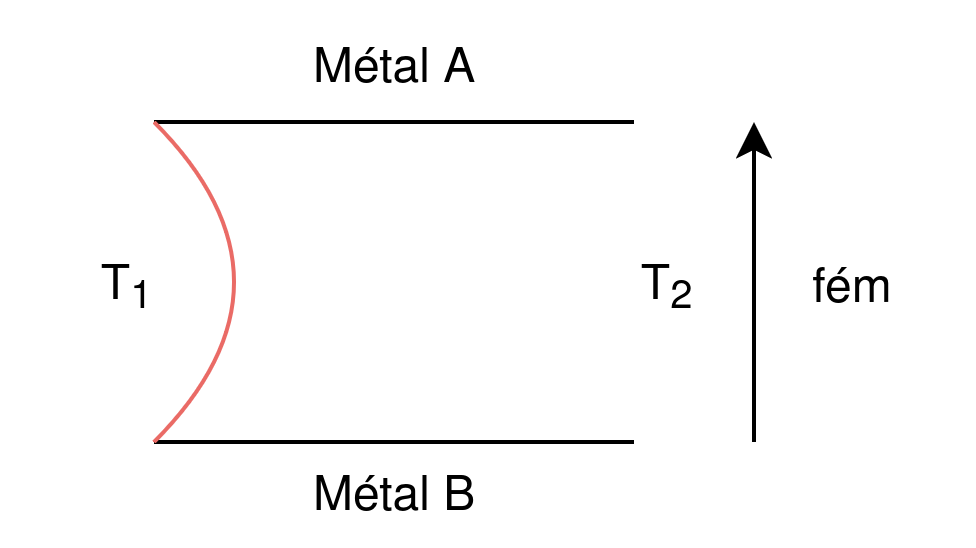
\includegraphics[width=0.9\textwidth]{thermoelectricite}
        \caption{Force électromotrice liée à la différence de température (\(T_1-T_2\))}
        \label{figThermoelectricite}
    \end{figure}
\end{minipage}
\begin{minipage}{0.5\textwidth}
    \begin{figure}[H]
        \centering
        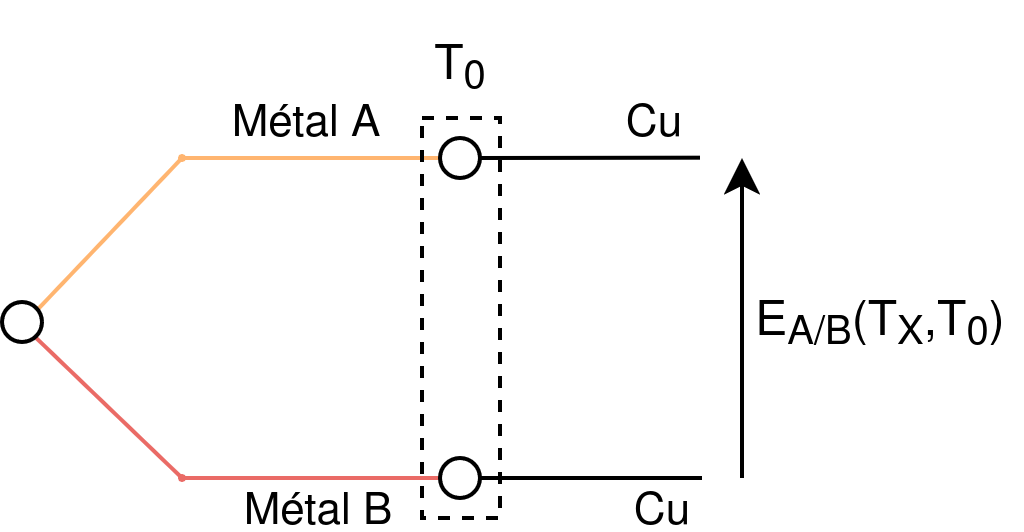
\includegraphics[width=0.9\textwidth]{thermocouple}
        \caption{Schéma d'un thermocouple}
        \label{figThermocouple}
    \end{figure}
\end{minipage}

Des tables normalisées permettent d'obtenir la f.é.m $E_{A/B}$ en fonction de la 
température $T_x$ lorsque $T_0$ est fixé à 0~°C.

\begin{figure}[H]
    \centering
    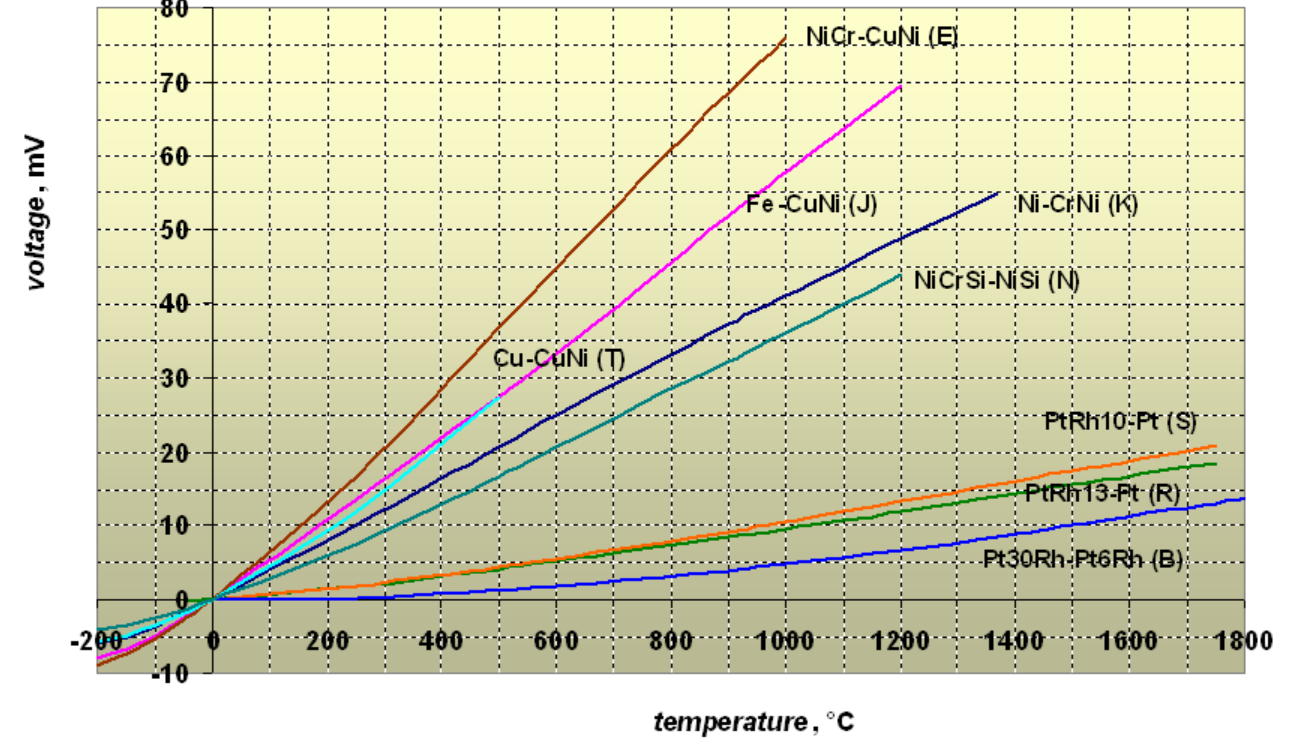
\includegraphics[width=0.9\textwidth]{thermocouple-graph}
    \caption{Variation de la différence de potentiel en fonction de la 
    température pour différents thermocouples.}
    \label{figThermocoupleGraph}
\end{figure}

D'un point de vue électronique, un thermocouple peut être modélisé selon le 
schéma de Thévenin, c'est-à-dire comme un générateur de tension en série avec 
une impédance $Z_c$.  

\begin{figure}[H]
    \centering
    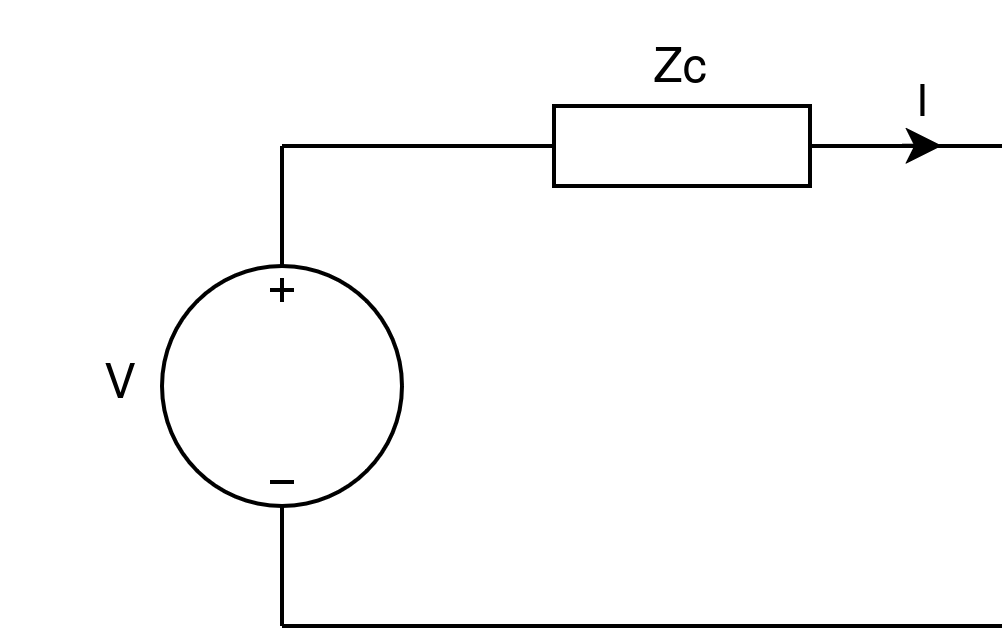
\includegraphics[width=0.5\textwidth]{thermocouple-Thevenin}
    \caption{Modèle de Thévenin d'un thermocouple}
    \label{figThermocoupleThevenin}    
\end{figure}

\subsection*{Pyroélectricité}
Certains cristaux présentent une polarisation spontanée dépendant de leur 
température. Lorsqu'ils absorbent un flux de rayonnement, leur température 
augmente, modifiant ainsi leur polarisation et entraînant une variation de 
tension détectable.  
Ce principe est exploité dans les capteurs pyroélectriques.

\begin{figure}[H]
    \centering
    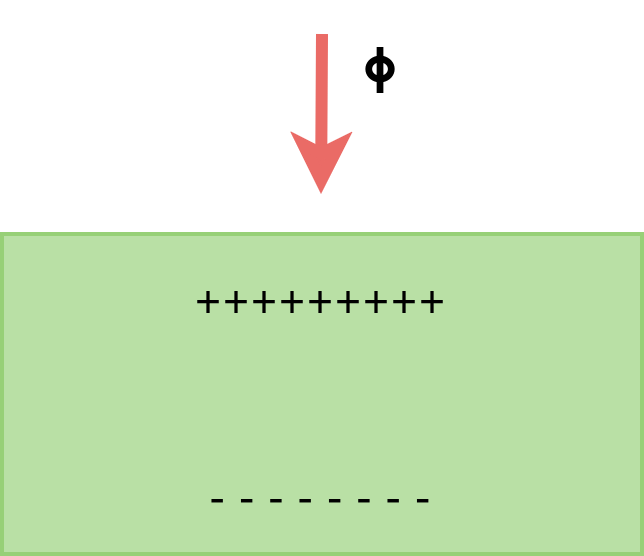
\includegraphics[width=0.3\textwidth]{pyroelectricite}
    \caption{Apparition de charges électriques}
    \label{figPyroelectricite}
\end{figure}

\subsection*{Piézo-électricité}
Certains cristaux, comme le quartz, se polarisent sous l'effet d'une contrainte 
mécanique. Cette déformation induit l'apparition de charges électriques sur les 
faces opposées du cristal.  
Ce phénomène est réversible, ce qui permet son utilisation dans divers capteurs 
piézoélectriques.

\begin{figure}[H]
    \centering
    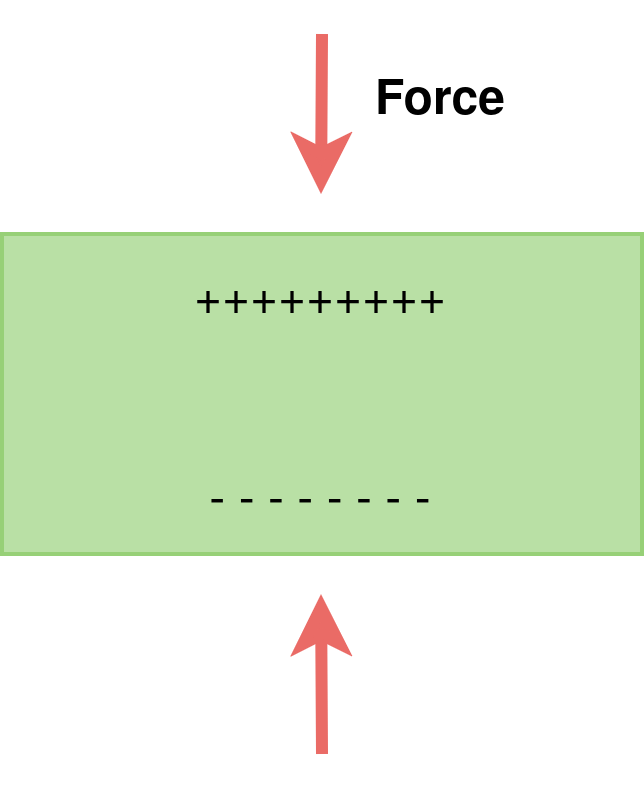
\includegraphics[width=0.3\textwidth]{piezoelectricite}
    \caption{Apparition de charges sur les faces opposées par la déformation du matériau.}
    \label{figPiezoelectricite}
\end{figure}

\subsection*{Photoélectricité}
Sous l'influence d'un rayonnement lumineux, certains matériaux libèrent des 
charges électriques. Ce principe est exploité dans les capteurs optoélectroniques
comme les photodiodes.

\begin{figure}[H]
    \centering
    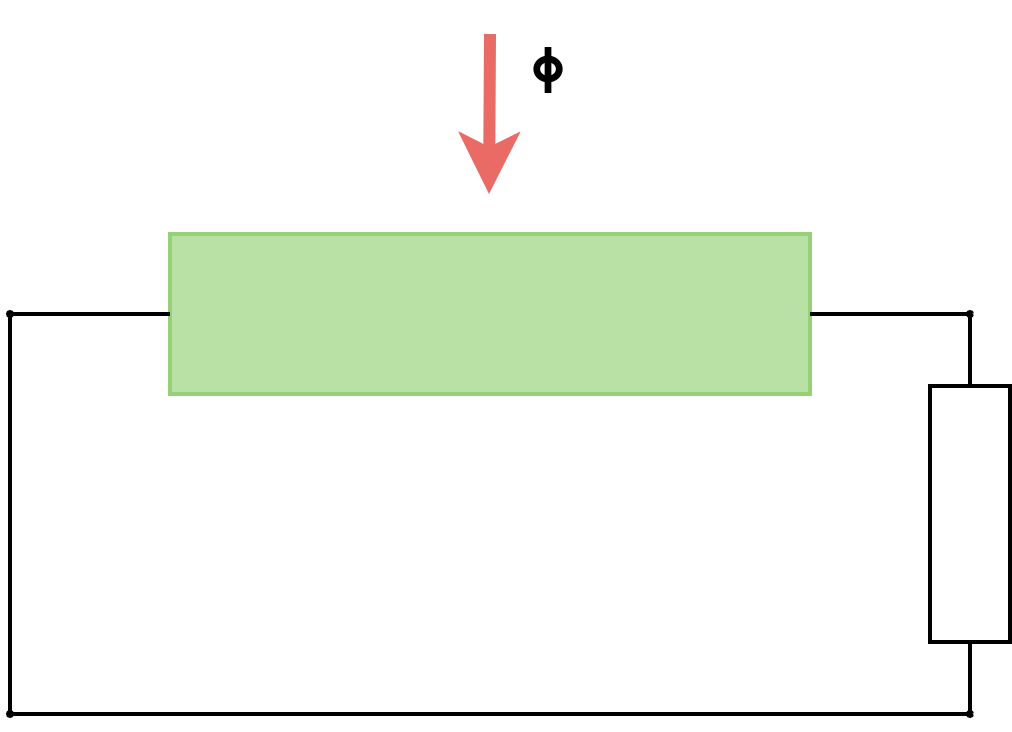
\includegraphics[width=0.4\textwidth]{photoelectricite}
    \caption{Apparition de charges sous l'effet de la lumière}
    \label{figPhotoelectricite}
\end{figure}

\subsubsection{Photodiode}
Une photodiode est un capteur générateur de courant. Elle est polarisée en 
inverse, ce qui signifie que le potentiel de l'anode est inférieur à celui de la 
cathode.  

Sans lumière, une photodiode est parcourue par un faible courant de fuite $I_0$. 
Lorsqu'un flux lumineux incident atteint la jonction de la diode, il génère un 
courant $I_\Phi$ par effet photoélectrique, s'ajoutant au courant de fuite. 
Ainsi, le courant total est donné par :
\[
I_d = I_0 + I_\Phi
\]

D'un point de vue électronique, une photodiode peut être modélisée par un schéma 
de Norton, c'est-à-dire comme un générateur de courant en parallèle avec une 
impédance $Z_D$. Ce modèle peut être précisé en ajoutant la source de courant de 
fuite $I_0$ et l'impédance $Z_D$, représentée par une résistance $R_D$ en 
parallèle avec une capacité $C_D$. Cette capacité correspond à l'accumulation 
des charges dans la photodiode lorsqu'elle est exposée à la lumière.

\begin{figure}[H]
    \centering
    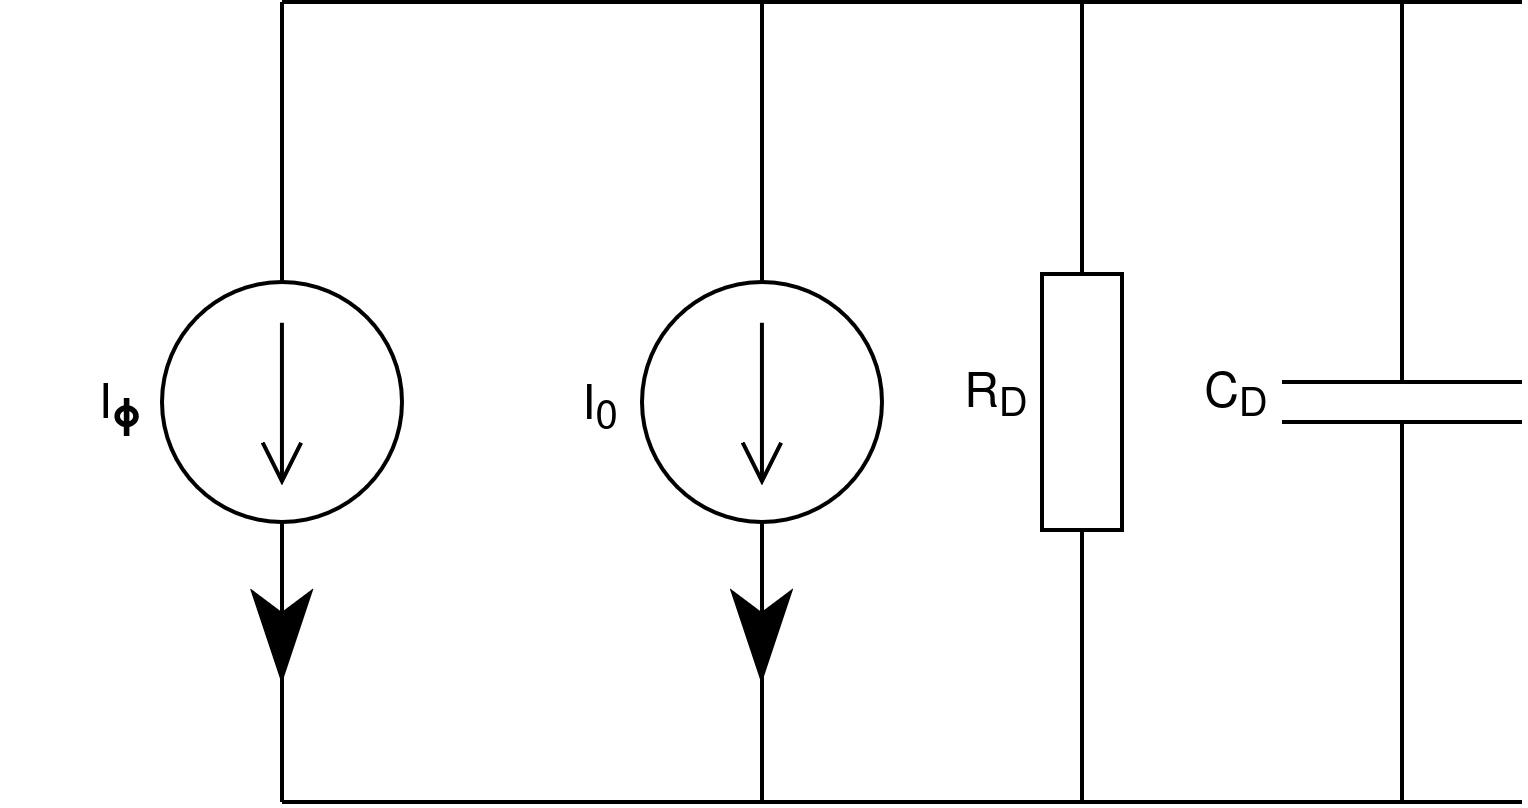
\includegraphics[width=0.7\textwidth]{photoelectricite-norton}
    \caption{Modèle de Norton d'une photodiode}
    \label{figPhotodiodeNorton}
\end{figure}

\subsection{Conditionnement des signaux des capteurs actifs}
Les capteurs actifs nécessitent souvent l'adjonction de conditionneurs pour améliorer l'exploitation de leur signal. Ces dispositifs permettent :
\begin{itemize}
    \item d'amplifier le signal lorsque son amplitude est trop faible ;
    \item de filtrer le signal pour supprimer les bruits parasites ou interférences ;
    \item d'adapter l'impédance afin d'assurer une meilleure transmission du signal ;
    \item de convertir le signal si nécessaire (ex~: conversion courant-tension, linéarisation) ;
    \item d'isoler électriquement le capteur du reste du circuit si besoin.
\end{itemize}

\subsection{Capteurs passifs}

\paragraph{Capteurs passifs}  
Les \textbf{capteurs passifs} sont des dispositifs qui ne génèrent pas 
directement de signal électrique, mais modifient une \textbf{grandeur électrique} 
telle que la \textbf{résistance} (\( R \)), l'\textbf{inductance} (\( L \)) ou 
la \textbf{capacité} (\( C \)) en réponse à une variation du \textit{mesurande}. 
En sortie, ils se comportent comme un \textbf{dipôle passif}, nécessitant ainsi 
un \textbf{circuit additionnel}, appelé \textit{conditionneur}, pour interpréter 
les variations de l'\textbf{impédance} et les convertir en un 
\textbf{signal exploitable}. Ce \textit{conditionneur} peut inclure des 
\textbf{ponts de mesure} (exemple : \textit{pont de Wheatstone} pour les 
capteurs \textbf{résistifs}), des \textbf{oscillateurs} (pour les capteurs 
\textbf{capacitifs}) ou des \textbf{circuits d'adaptation d'impédance} afin 
d'assurer une \textbf{lecture fiable et précise} des variations de la 
\textit{grandeur physique mesurée}.


\begin{table}[h]
    \centering
    \renewcommand{\arraystretch}{1.3}
    \renewcommand\tabularxcolumn[1]{m{#1}}
    \begin{tabularx}{\textwidth}{|>{\centering\arraybackslash}X|>{\raggedright\arraybackslash}X|>{\raggedright\arraybackslash}X|}
        \hline
        \textbf{Grandeur mesurée} & \textbf{Caractéristique électrique sensible} & \textbf{Types de matériaux utilisés} \\
        \hline
        Température & Résistivité électrique & Métaux : platine, nickel, cuivre … \\
        \hline
        Déformation & Résistivité électrique, Perméabilité magnétique & Alliage de Ni, Si dopé, Alliages ferromagnétiques \\
        \hline
        Position & Résistivité électrique & Magnétorésistances : bismuth… \\
        \hline
        Flux lumineux & Résistivité électrique & Semi-conducteurs \\
        \hline
        Humidité & Résistivité électrique & Chlorure de lithium \\
        \hline
    \end{tabularx}
    \caption{Caractéristiques électriques sensibles et matériaux utilisés pour différents capteurs}
    \label{tabCaracteristiquesCapteurs}
\end{table}

\subsection*{Capteurs résistifs}
Les capteurs résistifs sont des capteurs passifs dont la résistance varie en
fonction de la grandeur physique mesurée. Ils sont utilisés pour mesurer la
température, la pression, la déformation, l'humidité, etc.

\[
    R = f(a,b,c)/\sigma
\]

Avec \(f(a,b,c)\) une fonction de la géométrie et des dimensions \(a,b,c\) et 
\(\sigma\) la conductivit\'e du mat\'eriau.

Dans le cas spécifique d'un \textbf{capteur de température}, la 
\textbf{résistance} d'un matériau varie en fonction de sa \textit{température}.  
Il existe principalement deux types de capteurs de température :
\begin{itemize}
    \item \textbf{Les résistances métalliques}
    \item \textbf{Les thermistances}
\end{itemize}

\subsection*{Résistances métalliques (RTD - Résistance Température Detector)}

Les résistances métalliques ont une valeur \textbf{croissante} avec la 
température selon une loi d'évolution de la forme :
\begin{equation}
    R(T) = R_0 (1 + A T + B T^2 + C T^3)
\end{equation}
où :
\begin{itemize}
    \item \( T \) : température exprimée en \(^\circ C\)
    \item \( R_0 \) : résistance à \( 0^\circ C \)
    \item \( A, B, C \) : coefficients dépendant de la nature du métal
\end{itemize}

La \textbf{sonde de platine} est la plus utilisée et constitue un 
\textbf{étalon normalisé}. Cependant, d'autres matériaux comme le \textbf{Nickel} 
et le \textbf{Cuivre} sont aussi utilisés.

\subsection*{Caractéristiques de la sonde Platine}

\begin{itemize}
    \item Excellente \textbf{précision} sur une large gamme de température.
    \item Très bonne \textbf{stabilité} dans le temps.
    \item \textbf{Faible sensibilité} : environ \( 0.3 \) à \( 0.7 \, \Omega/^\circ C \).
    \item \textbf{Auto-échauffement} :
        \begin{itemize}
            \item Le courant échauffe la résistance, générant ainsi une erreur.
            \item Pour réduire cet effet, il faut utiliser un courant aussi faible que possible.
        \end{itemize}
    \item \textbf{Linéarisation} :
        \begin{itemize}
            \item La courbe de sortie \( R=f(T) \) est \textit{quasiment linéaire}.
        \end{itemize}
    \end{itemize}

\subsection*{Thermistances}

Les thermistances sont constituées de 
\textbf{mélanges agglomérés et frittés d'oxydes métalliques}. Leur 
\textbf{résistance décroît très rapidement} en fonction de la température selon 
la loi suivante :
\begin{equation}
    R(T) = R_0 \cdot e^{B \left( \frac{1}{T} - \frac{1}{T_0} \right)}
\end{equation}
où :
\begin{itemize}
    \item \( T \) : température exprimée en \( K \)
    \item \( R_0 \) : résistance à la température \( T_0 \)
    \item \( 3000K < B < 4000K \) : caractéristique de la thermistance
\end{itemize}

Les thermistances sont des \textbf{capteurs de grande sensibilité thermique} et 
sont particulièrement adaptées à la mesure de très faibles variations de 
température.

\subsection*{Types de thermistances}

Il existe deux types de thermistances selon leur réponse à la température :
\begin{itemize}
    \item \textbf{CTN} (\textit{Coefficient de Température Négatif}) : la résistance \textbf{diminue} lorsque la température \textbf{augmente}. Ces sondes peuvent être utilisées sur une large plage de température.
    \item \textbf{CTP} (\textit{Coefficient de Température Positif}) : la résistance \textbf{augmente} lorsque la température \textbf{augmente}.
\end{itemize}

\textbf{Linéarisation} : la réponse d'une thermistance 
\textit{n'est pas linéaire}. La variation de la résistance est beaucoup plus 
importante que pour une résistance métallique. D'où la nécessité d'un 
\textbf{conditionneur spécifique} pour linéariser la réponse.

\subsection{Capteurs résistifs}

Les \textbf{jauges d'extensométrie} sont des éléments \textbf{résistifs} qui 
peuvent être de nature \textit{métallique} ou \textit{semi-conductrice}.  

\begin{itemize}
    \item Ces jauges sont fixées sur un \textbf{support isolant mince}, lui-même \textbf{collé} à l'endroit de la structure dont on souhaite mesurer la \textit{déformation}.
    \item La variation de la résistance suit la relation :
\end{itemize}

\begin{equation}
    \frac{\Delta R}{R} = K \cdot \frac{\Delta l}{l}
\end{equation}

où :
\begin{itemize}
    \item \( \Delta R \) : variation de la résistance
    \item \( R \) : résistance initiale
    \item \( K \) : \textbf{facteur de jauge}
    \item \( \Delta l \) : variation de longueur de la structure
    \item \( l \) : longueur initiale
\end{itemize}

Les valeurs typiques du facteur de jauge \( K \) sont :
\begin{itemize}
    \item \textbf{Jauge métallique} : \( 2 < K < 4 \)
    \item \textbf{Jauge semi-conductrice} : \( \pm 50 < K < \pm 100 \)
\end{itemize}

La première application des jauges d'extensométrie est la 
\textbf{détermination des déformations} dans des 
\textit{structures soumises à des contraintes}.

\subsection*{Capteurs capacitifs}

Les \textbf{capteurs capacitifs} sont des \textbf{condensateurs}, généralement 
de \textit{forme plane} ou \textit{cylindrique}, dont la \textbf{capacité} est 
donnée par les relations suivantes~:

\begin{itemize}
    \item \textbf{Pour un condensateur plan}~:
    \begin{equation}
        C = \varepsilon_0 \varepsilon_r \cdot \frac{A}{d}
    \end{equation}
    
    \item \textbf{Pour un condensateur cylindrique}~:
    \begin{equation}
        C = 2 \pi \varepsilon_0 \varepsilon_r \cdot \frac{l}{\ln \left( \frac{r_2}{r_1} \right)}
    \end{equation}
\end{itemize}

où~:
\begin{itemize}
    \item \( C \)~: capacité du condensateur (\si{\farad})
    \item \( \varepsilon_0 \)~: \textbf{permittivité du vide} (\si{\farad\per\meter})
    \item \( \varepsilon_r \)~: \textbf{permittivité relative} du \textit{diélectrique}
    \item \( A \)~: \textbf{aire} des plaques du condensateur (\si{\meter\squared})
    \item \( d \)~: \textbf{distance} entre les plaques (\si{\meter})
    \item \( l \)~: \textbf{longueur} du condensateur cylindrique (\si{\meter})
    \item \( r_1, r_2 \)~: \textbf{rayons} intérieur et extérieur du condensateur cylindrique (\si{\meter})
\end{itemize}

Le \textbf{mesurande} agit sur la \textbf{capacité} en modifiant~:
\begin{itemize}
    \item la \textbf{permittivité} \( \varepsilon_r \) du \textit{diélectrique}
    \item les \textbf{dimensions géométriques} du condensateur (\( A, d, l, r_1, r_2 \))
\end{itemize}
